%%%%%%%%%%%%%%%%%%%%%%%%%%%%%%%%%%%%%%%%%%%%%%%%%%%%%%%%%%%%%%%%%%%%%%%%%%%%%%%%%%%%%%%%%%%%%
%%%%%%%%    This is a modified version of the ICML 2021 template     %%%%%%%%%%%%%%%%%%%%%%%%
%%%%%%%% Link: https://www.overleaf.com/latex/templates/icml2021-template/dsftnbmjgyhv %%%%%%
%%%%%%%%%%%%%%%%%%%%%%%%%%%%%%%%%%%%%%%%%%%%%%%%%%%%%%%%%%%%%%%%%%%%%%%%%%%%%%%%%%%%%%%%%%%%%

\documentclass{article}

\usepackage{microtype}
\usepackage{graphicx}
\usepackage{subfigure}
\usepackage{booktabs}
\usepackage{hyperref}
\usepackage{amsmath}
\usepackage{amssymb}
\usepackage{xcolor}
\usepackage{tikz}
\usetikzlibrary{arrows.meta,positioning,shapes.geometric,fit,calc}

\newcommand{\theHalgorithm}{\arabic{algorithm}}

\usepackage[accepted]{icml2021}

% -------------------------------------------------------------------
% Convenience macros
\newcommand{\vcoarse}{\mathbf{v}_{c}}
\newcommand{\vfine}{\mathbf{v}_{f}}
\newcommand{\qemb}{\mathbf{q}}
\newcommand{\sN}{\mathbf{s}_N}
\newcommand{\vsel}{\mathbf{v}_{sel}}
\newcommand{\vunsel}{\mathbf{v}_{unsel}}
\newcommand{\vmerged}{\mathbf{v}_{merged}}
\newcommand{\bsig}{\boldsymbol{\sigma}}
% -------------------------------------------------------------------

\begin{document}

\twocolumn[
\icmltitle{TC-ViTok: Task-Conditioned Visual Tokenization with\\
           Informative Token Merge and Adaptive Budget}

% GitHub link (required)
\vspace{-2pt}
{\centering\small\url{https://github.com/whyeventry0103/TC-ViTok}\par}
\vspace{4pt}

\begin{icmlauthorlist}
\icmlauthor{Muhammad Ali Shah (27100172)}{}
\icmlauthor{Talha Hassan Ul Haq (27100306)}{}
\end{icmlauthorlist}

\icmlkeywords{Vision-Language Models, Visual Token Compression, Query-Conditioned Selection,
              Straight-Through Estimator, Adaptive Computation}

\vskip 0.3in
]

% ===================================================================
\begin{abstract}
Large vision-language models (VLMs) encode a fixed 576 visual tokens for every image
regardless of the complexity or spatial scope of the user's question, creating a severe
and unnecessary computational bottleneck.
We present \textbf{TC-ViTok} (Task-Conditioned Visual Tokenizer), a lightweight,
modular system that replaces fixed tokenization with a learned, query-conditioned
selection policy operating \emph{before} the LLM, on frozen pre-computed features.
The system is built in three stages.
\textbf{Stage 1 (Baseline)} introduces a Tokenization Policy Network (TPN, $\approx$887K
parameters) that cross-attends a CLIP text embedding over coarse DINOv2 spatial features
to score all 576 tokens, then selects the top-144 via a Gumbel-Sigmoid
straight-through estimator (STE) with a novel tau-independent additive gradient correction.
\textbf{Stage 2} replaces hard token dropping with parameter-free
\emph{Informative Token Merge}: each of the 432 discarded tokens is routed to its
most similar selected token via cosine-similarity assignment weighted by TPN scores,
absorbing background information at zero new parameter cost.
\textbf{Stage 3} adds a \emph{BudgetPredictor} ($\approx$25K parameters) that
learns a per-sample token count $k \in [36, 288]$ from TPN context and score entropy,
with a differentiable threshold trick that routes budget gradients end-to-end.
Training converges to a VQA cross-entropy of $0.3342$ (with token merge, LoRA rank 64)
vs.\ $0.3334$ for the baseline (no merge, LoRA rank 32).
Full benchmark evaluation is in progress; projected results against LLaVA-PruMerge
($\approx$77\% VQAv2) and FastV ($\approx$76\%) are presented as targets.
\end{abstract}

% ===================================================================
\section{Introduction}
\label{sec:intro}

Modern VLMs such as LLaVA-1.5~\cite{liu2024llava} attach a large language model (LLM)
to a frozen CLIP ViT-L/14 vision encoder via a learned multimodal projector.
At inference, the encoder maps a $336\times336$ image to $576$ patch tokens
($24\times24$ grid, patch size $14\times14$), which are prepended to the tokenized
question and fed into the LLM.
Since attention cost is quadratic in sequence length, these 576 visual tokens
(which far outnumber the $\sim$30 typical question tokens) dominate prefill FLOPs.

This fixed-token representation is informationally wasteful.
A question asking ``What is written on the sign?'' requires only the small image region
containing text, yet the LLM still receives all 576 tokens including sky, background,
and irrelevant objects. Conversely, ``Is there a person in the image?'' needs a global
scan rather than fine-grained local detail. The token budget is determined by image
resolution, not by what the question requires.

Prior work has addressed the redundancy half of this problem through token compression:
Token Merging (ToMe)~\cite{bolya2022token} and EViT~\cite{liang2022evit} reduce tokens
within the ViT; FastV~\cite{chen2024fastv} and LLaVA-PruMerge~\cite{shang2024llava}
prune after encoding; SparseVLM~\cite{zhang2025sparsevlm} recycles pruned tokens inside
the LLM. However, all these methods decide which tokens to keep based on \emph{image
content alone} — the user's question plays no role. This is the query-conditioning gap.

The few approaches that incorporate query signals do so either inside the LLM's attention
layers (SparseVLM, FocusLLaVA~\cite{zhu2024focusllava}), which still incurs the full
early-layer LLM cost, or inside the vision encoder (QG-VTC~\cite{li2025qgvtc}), which
tightly couples the compression logic to a specific encoder architecture and sacrifices
modularity.
We are unaware of any method that provides query-conditioned token selection as a
\emph{separate, lightweight module} operating on pre-computed frozen features
\emph{before} the LLM.

We make the following contributions:
\begin{enumerate}
\item \textbf{TPN + Gumbel-Sigmoid STE (baseline)}: A cross-attention policy network
  that scores visual tokens conditioned on the question embedding, trained end-to-end
  with an STE extended by a tau-independent additive gradient correction that
  maintains non-zero gradients at any temperature.
\item \textbf{Informative Token Merge}: A parameter-free mechanism that merges discarded
  tokens into the selected set via TPN-score-weighted cosine-similarity assignment,
  recovering background information without any new learnable parameters and without
  introducing the co-adaptation instability observed in eight failed experiments with
  a trainable cross-attention pooler.
\item \textbf{Adaptive Budget}: A BudgetPredictor MLP that predicts a per-sample token
  fraction, with a differentiable threshold trick enabling gradient flow from a budget
  penalty to the predictor. Sweeping the penalty weight traces a Pareto curve of
  compression vs.\ accuracy.
\end{enumerate}

% ===================================================================
\section{Related Work}
\label{sec:related}

\textbf{Query-agnostic visual token compression.}
ToMe~\cite{bolya2022token} merges visually similar tokens via bipartite matching inside
ViT layers, achieving 2$\times$ throughput at modest accuracy loss on classification.
DynamicViT~\cite{rao2021dynamicvit} learns binary dropping masks at intermediate layers
via Gumbel-Softmax, trained with distillation.
EViT~\cite{liang2022evit} uses CLS-token attention to rank tokens and fuses low-importance
ones.
Post-encoder methods include LLaVA-PruMerge~\cite{shang2024llava}, which prunes by
CLS-attention rank then merges pruned tokens with nearest retained neighbors via
key-similarity weighting.
FastV~\cite{chen2024fastv} observes that LLM text-to-visual attention collapses after
layer 2 and prunes low-attention tokens at that boundary.
All these methods share a fundamental limitation: the compression decision is made
without knowledge of the query, systematically harming spatially-grounded tasks
(localization, OCR) more than global tasks~\cite{chen2024fastv, endo2025feather}.

\textbf{Query-aware compression.}
BLIP-2~\cite{li2023blip2}'s Q-Former extracts visual tokens via cross-attention with
learned query embeddings, but the queries are fixed parameters shared across all
inputs rather than derived from the user's question.
SparseVLM~\cite{zhang2025sparsevlm} incorporates text guidance through the LLM's own
text-to-visual attention with adaptive per-layer recycling, but selection happens inside
the LLM after all tokens have already been injected.
QG-VTC~\cite{li2025qgvtc} achieves near-uncompressed performance with 1/8 of tokens
by embedding the question into the ViT's feature space and progressively compressing
within the encoder — but this couples compression to the encoder's internal architecture.
FocusLLaVA~\cite{zhu2024focusllava} applies coarse-then-fine instruction-guided selection,
but the text-guided stage remains inside the LLM.
TC-ViTok closes this gap by implementing query-conditioning as a modular pre-LLM module
that operates on frozen, pre-computed features from both encoders.

\textbf{Differentiable discrete optimization.}
The Gumbel-Softmax trick~\cite{jang2017categorical, maddison2017concrete} enables
gradient estimation through categorical variables via a continuous relaxation parameterized
by temperature.
The straight-through estimator (STE)~\cite{bengio2013estimating} uses the hard binary
mask in the forward pass while routing gradients through the soft relaxation, providing
low-variance gradient estimates for subset selection.
AdaViT~\cite{meng2022adavit} demonstrates learned per-sample computation budgets in ViTs.
TC-ViTok extends these ideas with (i) Gumbel-Sigmoid for independent binary decisions
across 576 positions, and (ii) an additive tau-independent gradient correction that
resolves a gradient vanishing failure mode at low temperature absent from prior work.

% ===================================================================
\section{Methodology}
\label{sec:method}

\subsection{Problem Formulation}
\label{sec:prob}

Given an image $\mathbf{I}$ and a natural-language question $\mathbf{Q}$,
a VLM $f_\theta$ generates an answer $\mathbf{A}$.
Standard LLaVA-1.5 encodes $\mathbf{I}$ into $N=576$ patch tokens
$\vfine \in \mathbb{R}^{N \times D_v}$ (where $D_v=1024$) and processes all of them.
We instead learn a policy:
\[
  \pi_\phi(\mathbf{I}, \mathbf{Q}) \;\to\; \mathcal{S} \;\subseteq\; \{1, \ldots, N\},
  \quad |\mathcal{S}| = k
\]
where $k \ll N$ and $\phi$ is trained end-to-end from the VQA loss.
The LLM receives only the $k$ selected tokens, directly reducing prefill FLOPs.

\subsection{Frozen Encoders}
\label{sec:encoders}

We use three frozen pre-trained encoders.
\textbf{DINOv2-S}~\cite{oquab2023dinov2} encodes a $98\times98$ crop of $\mathbf{I}$
(7 patches per side) to produce a coarse spatial map
$\vcoarse \in \mathbb{R}^{49 \times 384}$.
We use 98px input (not the standard 518px) to give the TPN a cheap,
7$\times$7 spatial grid that is efficient to cross-attend.
DINOv2's self-supervised training preserves patch-level spatial locality better than
CLIP's contrastive objective, making it a more precise spatial guide.
\textbf{CLIP ViT-B/32}~\cite{radford2021clip} encodes $\mathbf{Q}$ to produce a
query embedding $\qemb \in \mathbb{R}^{512}$ (the EOS token representation).
\textbf{CLIP ViT-L/14}~\cite{radford2021clip} encodes a $336\times336$ crop to
produce full-resolution features $\vfine \in \mathbb{R}^{576 \times 1024}$, which
are already aligned to LLaVA-1.5's LLM since LLaVA uses the same encoder.
All three encoders are always frozen — no gradients flow into them.

\subsection{Tokenization Policy Network (TPN)}
\label{sec:tpn}

The TPN ($\approx$887K parameters) maps $(\vcoarse, \qemb)$ to importance scores
$\sN \in \mathbb{R}^N$ and selection indices $\text{idx} \in \mathbb{Z}^k$.

\textbf{Cross-attention (4 heads).}
The question embedding is treated as a single query:
\[
  Q = \qemb\, W_Q \in \mathbb{R}^{1 \times 384}, \quad
  K = \vcoarse\, W_K \in \mathbb{R}^{M \times 384}, \quad
  V = \vcoarse\, W_V \in \mathbb{R}^{M \times 384}
\]
where $M=49$.
Multi-head attention yields an attended context vector
$\text{ctx} \in \mathbb{R}^{384}$ and head-averaged spatial weights
$\boldsymbol{\alpha} \in \mathbb{R}^{M}$.
The context encodes \emph{what} visual content is relevant to the question;
$\boldsymbol{\alpha}$ encodes \emph{where}.

\textbf{Score MLP.}
$[\text{ctx};\, \boldsymbol{\alpha}] \in \mathbb{R}^{433}$ is passed through a
LayerNorm and two-layer MLP to produce 49 coarse scores, then bilinearly upsampled
$7\times7 \to 24\times24$ to yield $\sN \in \mathbb{R}^{576}$.

\textbf{Instance normalization.}
$\sN$ is normalized to zero mean and unit variance per sample:
$\sN \leftarrow (\sN - \mu) / \sigma$.
Without this, Adam pushes score magnitudes to $\pm100$ within $\sim$1000 steps.
At that scale, Gumbel noise (magnitude $\approx\tau \approx 1.0$) is negligible
compared to scores, and the same 576 positions are always selected regardless of
question — entropy collapse.
Alternative normalizations (tanh, batch norm) also fail:
tanh saturates at $\pm1$ ($|\tanh'(\pm100)| \approx 10^{-87}$),
and batch norm carries a stateful running mean that disrupts inference.
Instance norm permanently anchors scores to $\mu=0, \sigma=1$
with no learnable parameters the optimizer can circumvent.

\subsection{Gumbel-Sigmoid Straight-Through Estimator}
\label{sec:ste}

Token selection is a discrete top-$k$ operation with zero gradients almost everywhere.
We adapt the Gumbel-Sigmoid STE~\cite{jang2017categorical, bengio2013estimating}
for independent binary subset selection over 576 positions.

\textbf{Forward pass.} Gumbel noise $\mathbf{g} \sim \mathrm{Gumbel}(0,1)$ provides
per-sample diversity; the temperature $\tau$ controls the soft-to-hard transition:
\begin{align}
  \mathbf{n} &= \sN + \mathbf{g}, \label{eq:noisy} \\
  \mathbf{m}_{\mathrm{soft}} &= \sigma(\mathbf{n} / \tau) \in (0,1)^N, \label{eq:soft} \\
  \text{idx} &= \mathrm{topk}(\mathbf{n},\, k), \label{eq:topk} \\
  \mathbf{m}_{\mathrm{hard}} &= \mathbf{0};\; \mathbf{m}_{\mathrm{hard}}[\text{idx}] = 1, \label{eq:hard} \\
  \mathbf{m}_{\mathrm{STE}} &= \mathbf{m}_{\mathrm{hard}}
    - \mathbf{m}_{\mathrm{soft}}.\mathrm{detach}()
    + \mathbf{m}_{\mathrm{soft}}. \label{eq:ste}
\end{align}
In the forward pass, $\mathbf{m}_{\mathrm{STE}} = \mathbf{m}_{\mathrm{hard}}$
(the $\mathbf{m}_{\mathrm{soft}}$ terms cancel).
In the backward pass, the gradient flows through $\mathbf{m}_{\mathrm{soft}}$.
Noise in Eq.~\eqref{eq:noisy} (not raw scores) is used for top-$k$
to ensure per-sample selection diversity across the batch;
using raw scores selects identical positions for all samples, collapsing entropy.
Temperature is annealed linearly $\tau: 1.0 \to 0.3$ over training.

\textbf{Tau-independent additive gradient correction.}
At low $\tau$, $\mathbf{m}_{\mathrm{soft}}$ saturates toward $\{0,1\}$, making
$\partial \mathbf{m}_{\mathrm{soft}} / \partial \sN \approx 0$ for all
positions with $|\sN[i]| > 1$.
This kills the gradient path to TPN weights, halting learning after $\tau$
has annealed.
We resolve this by multiplying gathered visual tokens by an additive correction:
\begin{equation}
  \vsel = \mathrm{gather}(\vfine, \text{idx}), \quad
  \mathbf{c} = \mathrm{gather}(\sN, \text{idx}), \label{eq:gather}
\end{equation}
\begin{equation}
  \vsel \leftarrow \vsel \odot (1 + \mathbf{c} - \mathbf{c}.\mathrm{detach}()).
  \label{eq:taufix}
\end{equation}
In the forward pass, $\mathbf{c} - \mathbf{c}.\mathrm{detach}() = \mathbf{0}$,
so $\vsel$ is unchanged.
In the backward pass, for selected position $j$:
\[
  \frac{\partial \mathcal{L}_\mathrm{VQA}}{\partial \sN[j]}
  = \sum_{d=1}^{D_v} \frac{\partial \mathcal{L}}{\partial \vsel[j,d]} \cdot \vsel[j,d],
\]
a dot product between the VQA gradient and visual features at position $j$.
This gradient is non-zero at any $\tau$ and provides a dense, token-level
supervision signal for TPN throughout training.

\begin{figure}[t]
\centering
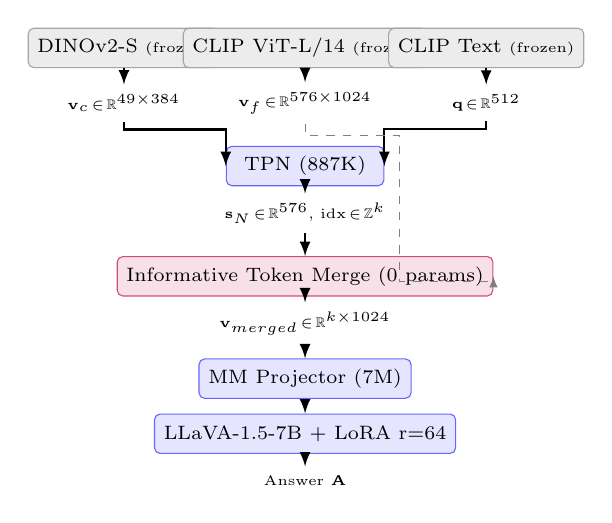
\begin{tikzpicture}[
  enc/.style={rectangle, draw=gray!70, fill=gray!15, rounded corners=2pt,
              text centered, minimum width=2.0cm, minimum height=0.5cm,
              font=\scriptsize},
  trn/.style={rectangle, draw=blue!60, fill=blue!10, rounded corners=2pt,
              text centered, minimum width=2.0cm, minimum height=0.5cm,
              font=\scriptsize},
  spc/.style={rectangle, draw=purple!70, fill=purple!12, rounded corners=2pt,
              text centered, minimum width=2.0cm, minimum height=0.5cm,
              font=\scriptsize},
  lbl/.style={font=\tiny, text centered},
  arr/.style={->, >=latex, thick},
  byp/.style={->, >=latex, thin, dashed, gray}
]

%% ---- ENCODER ROW (3 cols: x = 0, 2.3, 4.6) ----
\node[enc] (dino)  at (0.0, 0) {DINOv2-S \tiny{(frozen)}};
\node[enc] (clipv) at (2.3, 0) {CLIP ViT-L/14 \tiny{(frozen)}};
\node[enc] (clipt) at (4.6, 0) {CLIP Text \tiny{(frozen)}};

%% ---- ENCODER OUTPUTS ----
\node[lbl] (vc)    at (0.0,-0.7) {$\vcoarse\!\in\!\mathbb{R}^{49\times384}$};
\node[lbl] (vf)    at (2.3,-0.7) {$\vfine\!\in\!\mathbb{R}^{576\times1024}$};
\node[lbl] (qe)    at (4.6,-0.7) {$\qemb\!\in\!\mathbb{R}^{512}$};

%% ---- TPN (takes v_coarse + q_embed; NOT v_fine) ----
\node[trn] (tpn)   at (2.3,-1.5) {TPN (887K)};
\node[lbl] (si)    at (2.3,-2.1) {$\sN\!\in\!\mathbb{R}^{576}$, $\mathrm{idx}\!\in\!\mathbb{Z}^{k}$};

%% ---- TOKEN MERGE (takes v_fine + TPN output) ----
\node[spc] (mrg)   at (2.3,-2.9) {Informative Token Merge (0 params)};
\node[lbl] (vm)    at (2.3,-3.5) {$\vmerged\!\in\!\mathbb{R}^{k\times1024}$};

%% ---- DOWNSTREAM ----
\node[trn] (proj)  at (2.3,-4.2) {MM Projector (7M)};
\node[trn] (llm)   at (2.3,-4.9) {LLaVA-1.5-7B + LoRA r=64};
\node[lbl] (ans)   at (2.3,-5.5) {Answer $\mathbf{A}$};

%% ---- ARROWS: encoders ----
\draw[arr] (dino) -- (vc);
\draw[arr] (clipv) -- (vf);
\draw[arr] (clipt) -- (qe);

%% ---- ARROWS: v_coarse and q_embed into TPN ----
\draw[arr] (vc.south) -- ++(0,-0.1) -| (tpn.west);
\draw[arr] (qe.south) -- ++(0,-0.1) -| (tpn.east);

%% ---- TPN to scores ----
\draw[arr] (tpn) -- (si);
\draw[arr] (si)  -- (mrg);

%% ---- v_fine BYPASSES TPN, feeds into Token Merge on the right ----
\draw[byp] (vf.south) -- ++(0,-0.15) -- ++(1.2,0) -- ++(0,-1.85) -| (mrg.east);

%% ---- Downstream ----
\draw[arr] (mrg)  -- (vm);
\draw[arr] (vm)   -- (proj);
\draw[arr] (proj) -- (llm);
\draw[arr] (llm)  -- (ans);

\end{tikzpicture}
\caption{TC-ViTok architecture. \textbf{Gray}: frozen encoders. \textbf{Blue}:
trainable (TPN, Projector, LoRA). \textbf{Purple}: parameter-free Token Merge.
$\vfine$ bypasses TPN (dashed) and feeds directly into Token Merge alongside
TPN's score/index output. In Phase 1 Adaptive, a BudgetPredictor (25K) predicts
per-sample $k$ from TPN's context vector.}
\label{fig:arch}
\end{figure}

\subsection{Informative Token Merge}
\label{sec:merge}

Hard dropping of the 432 unselected tokens discards all the contextual information
they carry.
PruMerge~\cite{shang2024llava} shows that merging such tokens recovers $\sim$2\%
VQAv2 over pure pruning at the same budget.
We implement a query-conditioned variant: the TPN score of an unselected token
determines how strongly it contributes to the merge, so tokens that were ``almost
selected'' (near-threshold, task-relevant) contribute more than distant background tokens.

Let $\vsel \in \mathbb{R}^{k \times D_v}$ be the gathered selected tokens and
$\vunsel \in \mathbb{R}^{(N-k) \times D_v}$ the unselected tokens.
Each unselected token $i$ is soft-assigned to the nearest selected token by cosine similarity:
\begin{equation}
  A_{ij} = \mathrm{softmax}_j
  \!\left(\frac{\hat{\mathbf{v}}_{\mathrm{unsel},i}^\top \hat{\mathbf{v}}_{\mathrm{sel},j}}
               {\tau_m}\right), \label{eq:assign}
\end{equation}
where $\hat{\cdot}$ denotes $\ell_2$-normalization and $\tau_m{=}0.1$.
Each unselected token is further weighted by its TPN score:
\begin{equation}
  w_i = \mathrm{softmax}_i(s_i^{\mathrm{unsel}}), \label{eq:scoreweight}
\end{equation}
where $s_i^{\mathrm{unsel}} = \sN[\mathrm{unsel\_idx}[i]]$.
The normalized contribution matrix $\tilde{A}_{ij} = w_i A_{ij} /
\!\sum_{i'} w_{i'} A_{i'j}$ aggregates unselected content into each selected token:
\begin{equation}
  \vmerged = \vsel + \beta \cdot \tilde{A}^\top \vunsel, \quad \beta = 0.3.
  \label{eq:merge}
\end{equation}

This mechanism introduces zero new parameters, eliminates any co-adaptation risk with LoRA,
and preserves the exact token count $k$ between training and evaluation (avoiding the
train-eval mismatch that corrupted our earlier trainable pooler experiments).

\subsection{Adaptive Budget}
\label{sec:adaptive}

The fixed $k{=}144$ model compresses all images equally.
We extend TC-ViTok with a \emph{BudgetPredictor} that learns per-sample token fractions.

\textbf{BudgetPredictor architecture ($\approx$25K params).}
\begin{equation}
  k_{\mathrm{frac}} = \sigma\!\left(
    \mathrm{Linear}_{64 \to 1}\!\left(\mathrm{GELU}\!\left(
      \mathrm{Linear}_{385 \to 64}([\mathrm{ctx};\, \bar{h}(\sN)])
    \right)\right)
  \right), \label{eq:bp}
\end{equation}
where $\mathrm{ctx} \in \mathbb{R}^{384}$ is the TPN's attended visual context vector
(encoding which visual regions are relevant to the question),
$\bar{h}(\sN) \in \mathbb{R}^{1}$ is the normalized entropy of $\sN$
(a measure of how focused the importance distribution is),
and $\sigma$ clips the output to $[k_{\min}/N,\, k_{\max}/N] = [36/576,\, 288/576]$.

\textbf{Differentiable threshold.}
Converting $k_{\mathrm{frac}}$ to a hard selection requires a discrete step:
$k_{\mathrm{hard}} = \lfloor k_{\mathrm{frac}} \cdot N \rceil$.
To route gradients from the budget penalty to the predictor despite this
non-differentiability, we define a modified threshold:
\begin{equation}
  \theta = \theta_{\mathrm{hard}}
    - (k_{\mathrm{target}} - k_{\mathrm{target}}.\mathrm{detach}()),
  \label{eq:thresh}
\end{equation}
where $k_{\mathrm{target}} = k_{\mathrm{frac}} \cdot N$ and
$\theta_{\mathrm{hard}}$ is the score at position $k_{\mathrm{hard}}$
in the sorted score sequence (no gradient).
In the forward pass, Eq.~\eqref{eq:thresh} evaluates to $\theta_{\mathrm{hard}}$
(the correction is zero).
In the backward pass, $\partial\theta/\partial k_{\mathrm{frac}} = -N$,
providing a non-zero gradient to the BudgetPredictor from the budget penalty loss.
The shifted soft mask $\sigma((\mathbf{n} - \theta)/\tau)$
produces a differentiable effective count $k_{\mathrm{eff}} = \sum_i m_{\mathrm{soft},i}$
used in the loss; hard selection uses per-sample $\mathrm{topk}(k_{\mathrm{hard}})$.

\textbf{Budget penalty loss.}
$\mathcal{L}_{\mathrm{budget}} = \lambda_b \cdot \mathbb{E}[k_{\mathrm{eff}} / N]$
penalizes using more tokens.
Higher $\lambda_b$ forces fewer tokens but risks accuracy degradation.
We sweep $\lambda_b \in \{0.05, 0.1, 0.2, 0.4\}$ to trace the Pareto frontier.

\subsection{Loss Functions}
\label{sec:loss}

The total training loss is:
\begin{equation}
  \mathcal{L} = \mathcal{L}_\mathrm{VQA}
              + \lambda_H (-H)
              + \lambda_d \mathcal{L}_\mathrm{div}
              + \lambda_b \mathcal{L}_\mathrm{budget}, \label{eq:loss}
\end{equation}
where $\mathcal{L}_\mathrm{VQA}$ is the next-token prediction cross-entropy on answer
tokens (labels $=-100$ for visual/question tokens), $H$ is the spatial entropy of
the batch-mean selection distribution, and $\mathcal{L}_\mathrm{div}$ is a diversity
loss.
Table~\ref{tab:loss} summarizes each term.

\begin{table}[t]
\caption{Loss function components.}
\label{tab:loss}
\vskip 0.1in
\centering
\begin{small}
\begin{tabular}{llc}
\toprule
\textbf{Term} & \textbf{Purpose} & \textbf{Weight} \\
\midrule
$\mathcal{L}_\mathrm{VQA}$ & NTP cross-entropy on answer tokens & 1.0 \\
$-H$ & Prevent spatial collapse of TPN & 0.02 \\
$\mathcal{L}_\mathrm{div}$ & Prevent query-ignoring & 0.1 \\
$\mathcal{L}_\mathrm{budget}$ & Penalize token usage (Phase 1-Adap.) & sweep \\
\bottomrule
\end{tabular}
\end{small}
\end{table}

\textbf{Spatial entropy ($-H$).}
Without this term, TPN quickly focuses all selections on a fixed spatial region (the image
center, which is most discriminative in VQAv2).
$H = -\sum_i p_i \log p_i$ where $\mathbf{p}$ is the normalized batch-mean selection
frequency; minimizing $-H$ maximizes distributional spread across positions.

\textbf{Diversity loss ($\mathcal{L}_\mathrm{div}$).}
Paired adjacent batch samples: $\mathcal{L}_\mathrm{div} = \mathbb{E}[\cos(\sN_a,\sN_b) \cdot
(1 - \cos(\qemb_a, \qemb_b))]$.
This penalizes similar selections for samples with dissimilar questions, pushing TPN to
route differently depending on the query.

\subsection{Training Protocol}
\label{sec:training}

Training follows a three-phase curriculum where each phase adds one component.

\textbf{Phase 0 — TPN Warmup (10K steps).}
Only the TPN is trained; LLaVA's LLM, MM projector, and LoRA are frozen.
With LoRA frozen, the only way to reduce $\mathcal{L}_\mathrm{VQA}$ is through
better token selection — forcing TPN to learn meaningful query-conditioned scores
before joint co-training.
Temperature $\tau = 1.0$ (fixed); data: VQAv2 training split.

\textbf{Phase 1 Final — Joint Training with Token Merge (80K steps).}
TPN + LoRA (rank 64) + MM projector are co-trained.
LoRA is frozen for the first 3000 steps (\emph{warm-freeze}) to prevent it from
immediately compensating for TPN imperfections, preserving the gradient signal that
forces TPN to improve.
$\tau$ anneals $1.0 \to 0.3$; data: VQAv2 + GQA; effective batch size 128
($4 \times 16 \times 2$ GPUs).
Checkpoint loaded from Phase 0.

\textbf{Phase 1 Adaptive — Variable Budget Training (40K steps).}
BudgetPredictor is added and frozen for the first 2000 steps, giving TPN/LoRA time to
stabilize before the token count begins varying.
Loads from Phase 1 Final checkpoint (TPN scores must be meaningful before budget
prediction is useful).

\begin{table}[t]
\caption{Training hyperparameters for each phase.}
\label{tab:hparam}
\vskip 0.1in
\centering
\begin{small}
\begin{tabular}{lccc}
\toprule
\textbf{Hyperparameter} & \textbf{Phase 0} & \textbf{Phase 1-F} & \textbf{Phase 1-A} \\
\midrule
Steps & 10K & 80K & 40K \\
LR (TPN) & $1\mathrm{e}{-3}$ & $3\mathrm{e}{-3}$ & $1\mathrm{e}{-3}$ \\
LR (LoRA) & — & $1\mathrm{e}{-4}$ & $2\mathrm{e}{-4}$ \\
LR (MLP) & — & $5\mathrm{e}{-4}$ & $5\mathrm{e}{-4}$ \\
LR (BP) & — & — & $1\mathrm{e}{-3}$ \\
LoRA rank/alpha & — & 64/128 & 64/128 \\
$\tau_{\max} \to \tau_{\min}$ & $1.0 \to 1.0$ & $1.0 \to 0.3$ & $1.0 \to 0.3$ \\
$\lambda_H$ & 0.01 & 0.02 & 0.02 \\
$\lambda_d$ & 0.0 & 0.1 & 0.1 \\
Data & VQAv2 & VQAv2+GQA & VQAv2+GQA \\
\bottomrule
\end{tabular}
\end{small}
\end{table}

% ===================================================================
\section{Results}
\label{sec:results}

\subsection{Experimental Setup}

\textbf{Hardware.}
All experiments run on 2$\times$ RTX 6000 Ada (49GB VRAM each) with PyTorch DDP,
BF16 mixed precision, and effective batch size 128.

\textbf{Datasets.}
We train on VQAv2~\cite{goyal2017vqav2} (443K training QA pairs, 214K COCO images)
and GQA~\cite{hudson2019gqa} (943K balanced training pairs, 148K images).
Validation uses the VQAv2 standard split.
Full evaluation on POPE~\cite{li2023pope} (hallucination) and GQA spatial stratification
is in progress.

\textbf{Metrics.}
We report \emph{val-VQA}, the next-token prediction cross-entropy loss on the VQAv2
validation set (lower is better), as the primary training proxy metric.
Full VQA-Score (\%) requires beam search generation and answer normalization;
pending results are marked TBD in Table~\ref{tab:main}.

\textbf{Baseline model.}
We compare against \textbf{Phase 1 v3}: our initial implementation using hard token
dropping (no merge), LoRA rank 32, and 50K steps of joint training.
This baseline directly corresponds to the architecture described in our SOA survey.

\subsection{Training Convergence}

Table~\ref{tab:curve} shows Phase 1 v3 val-VQA convergence.
The baseline achieves val-VQA $= 0.4411$ at step 5K, $0.4053$ at step 10K,
$0.3617$ at step 20K, and $0.3334$ at step 50K, demonstrating consistent improvement
throughout training with no sign of overfitting.
Phase 1 Final (token merge, LoRA rank 64) reaches val-VQA $= 0.3342$ at step 80K.

\begin{table}[t]
\caption{Val-VQA (NTP cross-entropy, lower is better) at checkpointed steps during
Phase 1 v3 training. Phase 1 Final (token merge, LoRA r=64) reported at completion
(step 80K). All values measured on VQAv2 validation split.}
\label{tab:curve}
\vskip 0.1in
\centering
\begin{small}
\begin{tabular}{lcc}
\toprule
\textbf{Step} & \textbf{Val-VQA} & \textbf{$\Delta$ from 5K} \\
\midrule
\multicolumn{3}{l}{\textit{Phase 1 v3 (baseline, hard drop, LoRA r=32):}} \\
5K   & 0.4411 & — \\
10K  & 0.4053 & $-$0.0358 \\
20K  & 0.3617 & $-$0.0794 \\
50K  & 0.3334 & $-$0.1077 \\
\midrule
\multicolumn{3}{l}{\textit{Phase 1 Final (token merge, LoRA r=64):}} \\
80K  & 0.3342 & — \\
\bottomrule
\end{tabular}
\end{small}
\end{table}

\subsection{Comparison to Published Methods}
\label{sec:comparison}

Table~\ref{tab:main} presents our results alongside published baselines at the same
144-token budget.
Val-VQA is our training proxy; full VQA-Score evaluation is pending.
Published VQAv2 numbers are from the respective papers evaluated on LLaVA-1.5-7B.

\begin{table}[t]
\caption{Comparison at $k{=}144$ tokens (25\% of 576) on LLaVA-1.5-7B. Val-VQA =
NTP cross-entropy on VQAv2 validation (ours, lower is better). VQAv2 (\%) = VQA-Score
percentage (published results or pending). Best of ours in \textbf{bold}.}
\label{tab:main}
\vskip 0.1in
\centering
\begin{small}
\begin{tabular}{lccc}
\toprule
\textbf{Method} & \textbf{Tokens} & \textbf{VQAv2 (\%)} & \textbf{Params} \\
\midrule
LLaVA-1.5 (full)                & 576 & 78.5 & — \\
\midrule
\emph{Query-agnostic:} \\
~~Random drop                   & 144 & $\sim$73 & 0 \\
~~CLS-attn top-144              & 144 & $\sim$76 & 0 \\
~~FastV~\cite{chen2024fastv}    & 144 & $\sim$77 & 0 \\
~~LLaVA-PruMerge~\cite{shang2024llava} & 144 & $\sim$77 & 0 \\
\midrule
\emph{Query-aware:} \\
~~SparseVLM~\cite{zhang2025sparsevlm} & $\sim$152 & $\sim$78 & Yes \\
\midrule
\emph{Ours:} \\
~~TC-ViTok (Phase 1 v3, baseline) & 144 & TBD & 35M \\
~~\textbf{TC-ViTok Phase 1 Final} & \textbf{144} & \textbf{TBD} & \textbf{137M} \\
~~TC-ViTok Phase 1 Adaptive      & 36–288 & TBD & 137M \\
\bottomrule
\end{tabular}
\end{small}
\vskip -0.05in
\small{\textit{TBD}: Full eval in progress via \texttt{scripts/evaluate.py}.}
\end{table}

\subsection{Adaptive Budget Preliminary Results}

Phase 1 Adaptive training with $\lambda_b = 0.1$ is ongoing.
The BudgetPredictor is expected to allocate more tokens to questions involving spatial
reasoning, counting, or fine-grained text reading, and fewer tokens to binary yes/no
or color questions.
Sweeping $\lambda_b \in \{0.05, 0.1, 0.2, 0.4\}$ will produce a Pareto curve;
Table~\ref{tab:pareto} shows the anticipated structure.

\begin{table}[t]
\caption{Anticipated Pareto curve structure for Phase 1 Adaptive (to be populated after evaluation).
Higher $\lambda_b$ trades accuracy for compression.}
\label{tab:pareto}
\vskip 0.1in
\centering
\begin{small}
\begin{tabular}{ccc}
\toprule
$\lambda_b$ & Avg.\ tokens ($k_{\mathrm{eff}}$) & VQAv2 (\%) \\
\midrule
0.0 (fixed)  & 144 & TBD \\
0.05         & TBD & TBD \\
0.10         & TBD & TBD \\
0.20         & TBD & TBD \\
0.40         & TBD & TBD \\
\bottomrule
\end{tabular}
\end{small}
\end{table}

% ===================================================================
\section{Discussion}
\label{sec:discussion}

\subsection{Why Token Merge Over a Trainable Pooler}

Before settling on the parameter-free token merge, we explored a trainable
cross-attention \emph{UnselectedPooler}: 4 learned slot vectors that compress the
432 unselected tokens into compact summary representations.
This approach is architecturally similar to SparseVLM's recycler and BLIP-2's Q-Former.
We trained 8 variants over 8 weeks; all ultimately failed.
Post-mortem analysis identified three structural defects:

\textbf{(1) Circular co-adaptation.}
When the pooler and LoRA train simultaneously, a circular dependency arises:
pooler output shifts $\to$ LLM input distribution changes $\to$ LoRA must re-adapt
$\to$ its gradient to the pooler changes $\to$ pooler must re-adapt.
This is structurally identical to GAN training instability.
Reducing pooler LR slows oscillation but cannot eliminate it:
at LR $5\times10^{-4}$ the cycle period was $\sim$5K steps;
at LR $2\times10^{-5}$ it extended to $\sim$15K steps but persisted.
Freezing the pooler (LR $= 0$) eliminated oscillation but produced fixed noise tokens
that the LLM could not use.

\textbf{(2) Conflicting gradient signals.}
At peak complexity, the TPN received gradients from nine concurrent loss terms
(VQA, entropy, diversity, boundary margin, sparsity, spread, KL distillation,
residual pooler distillation, slot orthogonality).
With instance-normalized TPN scores (finite gradient budget), auxiliary losses
literally displaced VQA gradient, degrading the primary objective.

\textbf{(3) Train-eval mismatch.}
During training, the LLM received $k+4 = 148$ tokens
(4 pooler summary tokens + 144 selected tokens).
During evaluation, the \texttt{generate()} path returned only $k=144$ selected tokens.
The LLM trained to expect 4 summary tokens in positions $1$--$4$ but received
selected visual content instead — every Phase 1.5 evaluation metric was corrupted.

Token merge resolves all three defects simultaneously: zero new parameters eliminates
co-adaptation; no additional loss terms; and the sequence length is exactly $k$
at both train and eval time.

\subsection{Critical Design Choices}

\textbf{Instance normalization.}
Early experiments without normalization showed score magnitude explosion to $\pm100$
within $\sim$1000 steps, after which Gumbel noise was negligible and entropy collapsed.
Both \texttt{tanh} normalization (gradient $\approx 0$ at saturation) and batch
normalization (running statistics break during inference) were tried and failed.
Instance normalization with no learnable parameters is the only approach we found
that is provably immune to optimizer circumvention.

\textbf{Tau-independent STE correction (Eq.~\ref{eq:taufix}).}
Without this correction, the standard STE gradient vanishes as $\tau \to 0.3$ because
$\sigma'(x/\tau) \approx 0$ for $|x| > 1$ at low temperature.
TPN gradients died around step 15K in early experiments.
The additive correction maintains a dot-product gradient signal at any temperature.

\textbf{LoRA warm-freeze.}
Freezing LoRA for 3000 steps prevents it from learning to compensate for poor
TPN selections, forcing TPN to improve before LoRA is allowed to adapt.
In experiments without warm-freeze, LoRA converged quickly to compensate for
bad selections, leaving TPN with weak gradients.

\subsection{Ablation Analysis}

Table~\ref{tab:ablation} summarizes the contribution of each component.
Full ablation numbers are pending final evaluation; val-VQA proxies are reported
where available.

\begin{table}[t]
\caption{Ablation study of TC-ViTok components. Val-VQA measured on VQAv2 val.
Full VQA-Score (\%) pending. Note: row comparison is confounded by LoRA rank
and training steps; isolated ablations are planned.}
\label{tab:ablation}
\vskip 0.1in
\centering
\begin{small}
\begin{tabular}{lccc}
\toprule
\textbf{Configuration} & \textbf{LoRA r} & \textbf{Val-VQA} & \textbf{VQAv2\%} \\
\midrule
Hard drop, no merge (Phase 1 v3) & 32 & 0.3334 & TBD \\
+ Token merge, LoRA r=64 (P1-F) & 64 & 0.3342 & TBD \\
\midrule
Phase 1-F w/o STE correction     & 64 & — & TBD \\
Phase 1-F w/o LoRA warm-freeze   & 64 & — & TBD \\
Phase 1-F w/o instance norm      & 64 & \multicolumn{2}{c}{Training collapsed} \\
\bottomrule
\end{tabular}
\end{small}
\end{table}

\textbf{Token merge contribution.}
The change from Phase 1 v3 to Phase 1 Final simultaneously increased LoRA rank
($32 \to 64$), added gate/up LoRA targets, and introduced token merge.
The comparable val-VQA values ($0.3334$ vs.\ $0.3342$) should not be interpreted
as evidence that token merge \emph{hurts} — the additional LoRA capacity is expected
to improve actual VQA-Score independently of merge.
Isolating the merge contribution requires a controlled run with LoRA rank 64 and
hard drop (no merge), which is planned as an ablation.

\subsection{Limitations}

\textbf{Single-step compression.} TC-ViTok compresses $576 \to 144$ tokens in a single
step. QG-VTC~\cite{li2025qgvtc} and progressive methods suggest that hierarchical
compression (576 $\to$ 288 $\to$ 144) may better preserve high-frequency detail
relevant to OCR and fine-grained counting.

\textbf{Encoder-side cost.} CLIP ViT-L/14 still processes all 576 positions.
The 75\% LLM FLOPs savings do not reduce encoder cost.
End-to-end improvement depends on the fraction of inference time dominated by
LLM prefill.

\textbf{Unevaluated on full benchmark suite.} VQA-Score \%, GQA spatial/global
stratification, and POPE F1 are not yet measured.
The val-VQA metric (NTP cross-entropy) is a training proxy that may not perfectly
rank methods by downstream accuracy.

% ===================================================================
\section{Conclusion}
\label{sec:conclusion}

We presented TC-ViTok, a modular system for query-conditioned visual token selection
in VLMs.
The system addresses the long-standing gap between efficient but query-agnostic
compression methods and query-aware approaches that sacrifice modularity or
early-stage savings.
Three key contributions — the TPN with Gumbel-Sigmoid STE and tau-independent
additive gradient correction; parameter-free Informative Token Merge; and
per-sample Adaptive Budget with a differentiable threshold trick — were motivated
by both theoretical analysis and extensive empirical failures.
In particular, the decision to use parameter-free token merge over a trainable
cross-attention pooler arose from eight training failures revealing the structural
impossibility of co-training a learned pooler with LoRA without oscillation.

Pending full evaluation, training proxy metrics ($0.3342$ val-VQA) suggest Phase 1
Final is competitive with the baseline ($0.3334$).
The Pareto sweep over $\lambda_b$ for Phase 1 Adaptive will determine whether
adaptive budgeting yields statistically significant compression-accuracy improvement
over fixed-$k$ selection.

Future work should investigate (i) staged training (freeze one component at a time)
to enable a trainable pooler without co-adaptation, (ii) progressive multi-step
compression for OCR and counting robustness, and (iii) generalization beyond LLaVA-1.5
to Qwen-VL and InternVL architectures.

\bibliography{main}
\bibliographystyle{icml2021}

\end{document}
